\documentclass[style=husky,clock,size=9pt,dvipsnames]{powerdot}
\usepackage[utf8]{inputenc}
\usepackage{amssymb}
%\usepackage{eqnarray,amsmath} % already loaded by mathtools below
\usepackage{mathtools}
\usepackage{mathrsfs}
\usepackage{pifont}
\usepackage{latexsym}
\usepackage{hyperref}
\usepackage{array, booktabs}
\usepackage{chronosys}
\usepackage{animate}
\usepackage{fourier}
%\usepackage[]{xcolor}
\usepackage{multirow}
\usepackage{multicol}
%\usepackage[export]{adjustbox}% http://ctan.org/pkg/adjustbox
%\usepackage{wrapfig} % wrap text around figures and tables BUT DOESN'T WORK WITH LISTS

\newcounter{savedenum}
\newcommand*{\saveenum}{\setcounter{savedenum}{\theenumi}}
\newcommand*{\resume}{\setcounter{enumi}{\thesavedenum}}

\usepackage{tcolorbox} % color boxes 

\usepackage{charter}
\usepackage{environ}
\usepackage{tikz}
\usetikzlibrary{matrix}
\usetikzlibrary{calc,positioning,shadows.blur,decorations.pathreplacing,tikzmark,fit,shapes.geometric}
%\usepackage{etoolbox}
\usepackage{ifpdf}
\usetikzlibrary{shapes,calc}
\usepackage{pdfpages}
\usepackage{graphicx}
%\usepackage{bmpsize}
\usepackage{colortbl}
\usepackage{bbding}
%\DeclareCaptionFont{blue}{\color{LightSteelBlue3}}% light blue color for timeline
%\DeclareGraphicsExtensions{.pdf,.png,.jpg}
\ifpdf
%
\else
% Implement Outline text using pstricks if regular LaTeX->dvi->ps->pdf route
\usepackage{pst-all}
\fi

%%%%%%%%%%%%%%%
%GET CUSTOM BLOCKS
%%%%%%%%%%%%%%%
\tcbuselibrary{skins}
\definecolor{myblue}{rgb}{0.15,0.15,0.53}

\makeatletter

\newtcbox{\titlebox}{
	enhanced,
	overlay={
		\draw[myblue,fill=myblue](frame.south east)--+(0,.2)to[bend right]+(.2,-0)--cycle;},
	colback=myblue,
	top=-1pt,bottom=-2pt,left=2pt,right=2pt,
	boxrule=1pt,
	colframe=myblue,
	sharp corners=south,
	colupper=white,
	fontupper=\bfseries
}

\newtcolorbox{myblock}[1][]{
	enhanced,
	left=2pt,
	right=2pt,
	colframe=myblue,
	boxrule=1pt,
	colback=blue!10,
	overlay={
		\def\myblock@tempa{#1}
		\ifx\myblock@tempa\@empty
		\else
		\draw[myblue,fill=myblue]($(frame.north west)+(.2pt,-.2pt)$)--+(.1,0)to[bend right]+(-0,-.1)--cycle;
		\node [
		anchor=south west,
		inner sep=0pt,
		outer sep=0pt
		]at(frame.north west){\titlebox{#1}};
		\fi
	},
}
\makeatother

%%%%%%%%%%%%%%%%%%%%%
%%% Red tcolorbox with pink background 
%%%%%%%%%%%%%%%%%%%%%
\newtcolorbox{mytcolorbox}[2][]{colback=red!5!white,colframe=red!75!black,title=#2,#1}

%%%%%%%%%%%%%%%%%%%%%%%%%%%%%
%%% Red tcolorbox with pink background (inline version)
%%%%%%%%%%%%%%%%%%%%%%%%%%%%%
\newtcolorbox{myinlinetcb}[2][]{colback=red!5!white,
	colframe=red!75!black,fonttitle=\bfseries,hbox,
	title=#2,top=0pt,bottom=0pt,left=0pt, right=0pt,#1,nobeforeafter,box align=base}

%%%%%%%%%%%%%%%%%%%%%
%%% Red tcbox with pink background 
%%%%%%%%%%%%%%%%%%%%%
\newtcbox{\mytcbox}[1]{colback=red!5!white,
	colframe=red!75!black,fonttitle=\bfseries,
	title=#1}

%%%%%%%%%%%%%%%%%
% Basic diagrams style
%%%%%%%%%%%%%%%%%
%\usetikzlibrary{arrows, arrows.meta,positioning} 
%\tikzset{
%    %Define standard arrow tip
%    >=stealth',
%    %Define style for xes
%    punkt/.style={
%           rectangle,
%           rounded corners,
%           draw=black, very thick,
%           text width=6.5em,
%           minimum height=2em,
%           text centered},
%    % Define arrow style
%    pil/.style={
%           ->,
%           thick,
%           shorten <=2pt,
%           shorten >=2pt,}
%}

%%%%% TICKS %%%%%%%
\newcommand*\tick{\item[\Checkmark]}
\newcommand*\fail{\item[\XSolidBrush]}

\newcommand*\ef{\mathscr{E}} % Electric Field
\newcommand\ra{$\rightarrow$} % Right arrow
\newcommand\lra{$\longrightarrow$} % long Right arrow
\newcommand\Lra{$\Longrightarrow$} % Long Right arrow
\newcommand\myred{\textcolor{Red}} % Red text
\newcommand*\myblue{\textcolor{Blue}} % Red text
\newcommand\mygreen{\textcolor{Green}} % Red text
%%%%% GET ALGORITHMS LIKE EXPRESSIONS %%%%%%%
\usepackage[linesnumbered,ruled,vlined]{algorithm2e} 

\title{Particle Detector Systems}
\author{Alfredo D. Ferella}
\date{2018/02/05}
 
\begin{document}
 
\maketitle
 
\begin{slide}[toc=,bm=]{Overview}
	\tableofcontents[content=sections]
\end{slide}

\section{Momentum reconstruction - Particle Tracking}
\begin{wideslide}[trans=Fly,toc=]{Motivation for tracking detectors}
\twocolumn[lcolwidth=0.5\textwidth]{
  \begin{itemize}
  \item Main purpose: measure \red{coordinates} of charged particles with high precision in a magnetic field
  \item Measure the curvature $\rightarrow$ \red{momentum}
  \item Curvature measurement requires the reconstruction of track patterns in an
  ensemble of measured hits in detectors $\rightarrow$ \mygreen{pattern recognition (reconstruction software)}\\
  hits \ra coordinates \ra tracks \ra momentum
  \item Additional tasks: \red{vertex reconstruction} extrapolate tracks back to their origin \ra primary vertex at the interaction point or secondary vertex
  \item Determination of impact parameter w.r.t. primary vertex \ra \red{lifetime tags (b-tagging)}
  \end{itemize}
}
{\begin{figure}
	\includegraphics[width=\textwidth]{Figures/h_to_4e}
\end{figure}
}
\end{wideslide}

\begin{wideslide}[trans=Fly,toc=]{Momentum reconstruction}
\twocolumn[lcolwidth=0.5\textwidth]
	{Equation of motion: }
	{\(\vec{F}=m\cdot\gamma\cdot\vec{a}=q\left(\vec{v}\times\vec{B}\right)\)}
\vspace{0.2cm}
\twocolumn[lcolwidth=0.5\textwidth]
	{Second order differential equation:}
 	{\(\ddot{\vec{x}}=\frac{q}{m\cdot\gamma}\dot{\vec{x}}\times\vec{B}(x)\)}
Two types of accelerator setups:\\
\vspace{0.5cm}
\twocolumn[lcolwidth=0.6\textwidth,rcolwidth=0.4\textwidth]
	{Fixed target:
	\begin{figure}
		\includegraphics[width=\textwidth]{Figures/fixed_target}
	\end{figure}
	Measured coordinates: $x(z_i)$, $y(z_i)$\\
	}
	{Collider :
		\begin{figure}
			\includegraphics[width=\textwidth]{Figures/collider}
		\end{figure}
	$\phi(z_i)$, $r(z_i)$
	}
Usually $\vec{B}$ is homogeneous \ra circular orbit of curvature radius $\rho$:
\begin{minipage}{0.4\linewidth}
	\[
		\frac{mv^2}{\rho}=q\vec{v}\times\vec{B}=qv_\perp\cdot|\vec{B}|
	\]
\end{minipage}
\begin{minipage}{0.25\linewidth}
	\[
		\rho=\frac{p^2}{qp_\perp B}
	\]
\end{minipage}
\begin{minipage}{0.25\linewidth}
	\begin{mytcolorbox}[top=-1pt,bottom=-2pt,left=2pt,right=2pt]{If $\vec{p}\perp\vec{B}$ - Forward}
		\[
			\rho=\frac{p}{qB}
		\]
	\end{mytcolorbox}
\end{minipage}

\end{wideslide}

\subsection{Forward Spectrometer}
\begin{wideslide}[trans=Fly,toc=]{Forward Spectrometer}
	Configuration of mainly fixed target (but also LHCb) or ALICE forward muon spectrometer
	\begin{figure}
		\includegraphics[width=0.75\linewidth]{Figures/forward_spect}
	\end{figure}
The magnetic field gives (additional) $p_\perp$-kick $\Delta p_\perp$\\
Typically $p \gg p_\perp$, $\Delta p_\perp$ \ra Lorentz force always approximately in x-direction and
\twocolumn[lcolwidth=0.4\linewidth,rcolwidth=0.4\linewidth]
	{
		\begin{equation*}
		\Delta p_\perp=q\rho B_y L
		\end{equation*}
		For uniform B
	}
	{
		\begin{equation*}
		\Delta p_\perp=q\rho \int_{L}B dL
		\end{equation*}
		For variable B
	}
\end{wideslide}

\begin{wideslide}[trans=Fly,toc=]{Forward Spectrometer - Precision }		
	\twocolumn[]
	{
		Usually $\rho\gg L$ \ra
		\[
			\theta\approx\frac{L}{\rho}=\frac{L}{p}qB_y
		\]
		\[
			\Delta p_x=p\sin\theta\approx p\theta=LqB_y
		\]
		\[
			\mbox{or}\qquad\approx q\int_0^{L}B_ydL
		\]
	}
	{
		\begin{figure}
			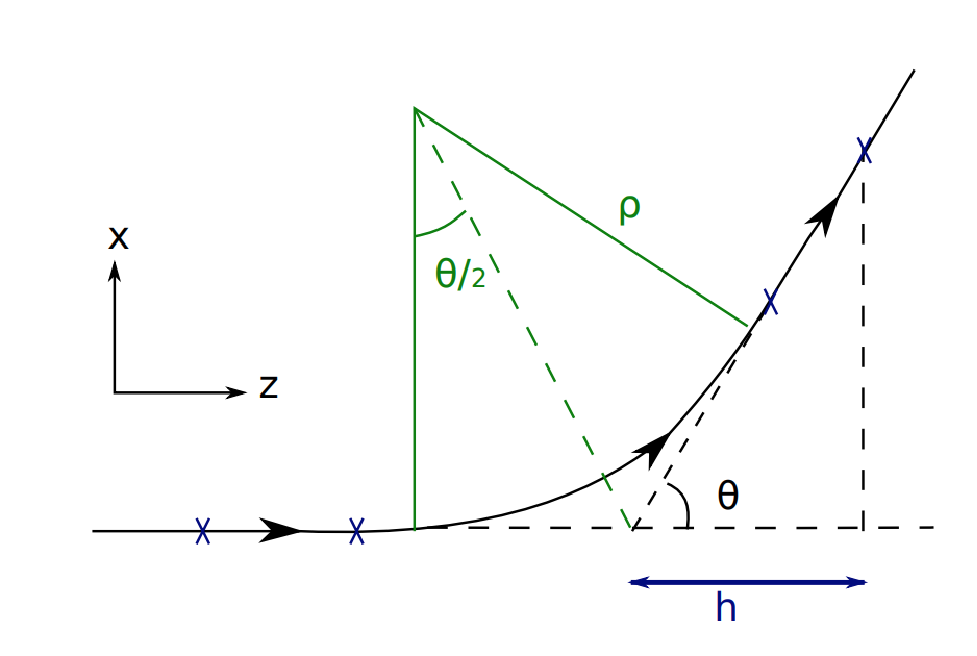
\includegraphics[width=\linewidth]{Figures/track_deflection}
		\end{figure}
	}
\end{wideslide}

\section{Calorimetry}
\begin{slide}[trans=Fly,toc=]{Calorimetry}
	\begin{myblock}{}
		Calorimetry: = \myred{Energy} measurement by total absorption,
		usually combined with spatial information / reconstruction
	\end{myblock}
	\begin{itemize}
		\item 
		In addition: most calorimeters are position sensitive, i.e. segmented, to measure
		\begin{itemize}
			\item The \myred{position} of the energy deposition (cell structure, $\eta-\phi$ position)
			\item The \myred{direction} of the incoming particle (requires in addition longitudinal
				segmentation)
		\end{itemize}
		and finally: calorimeters contribute to \myred{particle identification}
		(type of interaction \ra form of energy deposition)
	\end{itemize}
\end{slide}

\begin{slide}[trans=Fly]{Operation Principles}
	\begin{itemize}
		\item
		Energy is transferred to an electrical signal (ionization charge or to a light signal - scintillation or Cherenkov)
		\item 
		This signal should be proportional to the original energy: $E =\alpha S$\\
		Calibration procedure \ra $\alpha$ [GeV/$S$]
		\item
		Energy of primary particle is transferred to new particles\\
		\ra cascade / shower of new, lower energy particles
	\end{itemize}
		The shower development is determined by the type of the incoming particle and the corresponding interaction;\\
		One distinguishes between electromagnetic showers (e,$\gamma$) and hadronic showers (initiated by all hadrons, inelastic hadronic interactions)
		\begin{figure}
			\includegraphics[width=0.4\textwidth]{Figures/em_calorimeter}
			\includegraphics[width=0.4\textwidth]{Figures/hadr_calorimeter}
		\end{figure}
\end{slide}

\begin{slide}[trans=Fly]{Calorimeter Layouts}
	\begin{enumerate}
		\item  \mygreen{Homogeneous calorimeter}\\
		One material serves to absorb the energy and to provide the measureable signal
		(e.g. lead glass block, scintillator block, liquid argon volume)\\
		\includegraphics[width=0.4\textwidth]{Figures/homogeneous_calor}
		\item 
		\mygreen{Sampling calorimeter}\\
		Absorber material (passive) (Fe, Pb, Cu, ...)\\
		+ Sensitive detector medium (Liquid/gas ionisation or scintillation)\\
		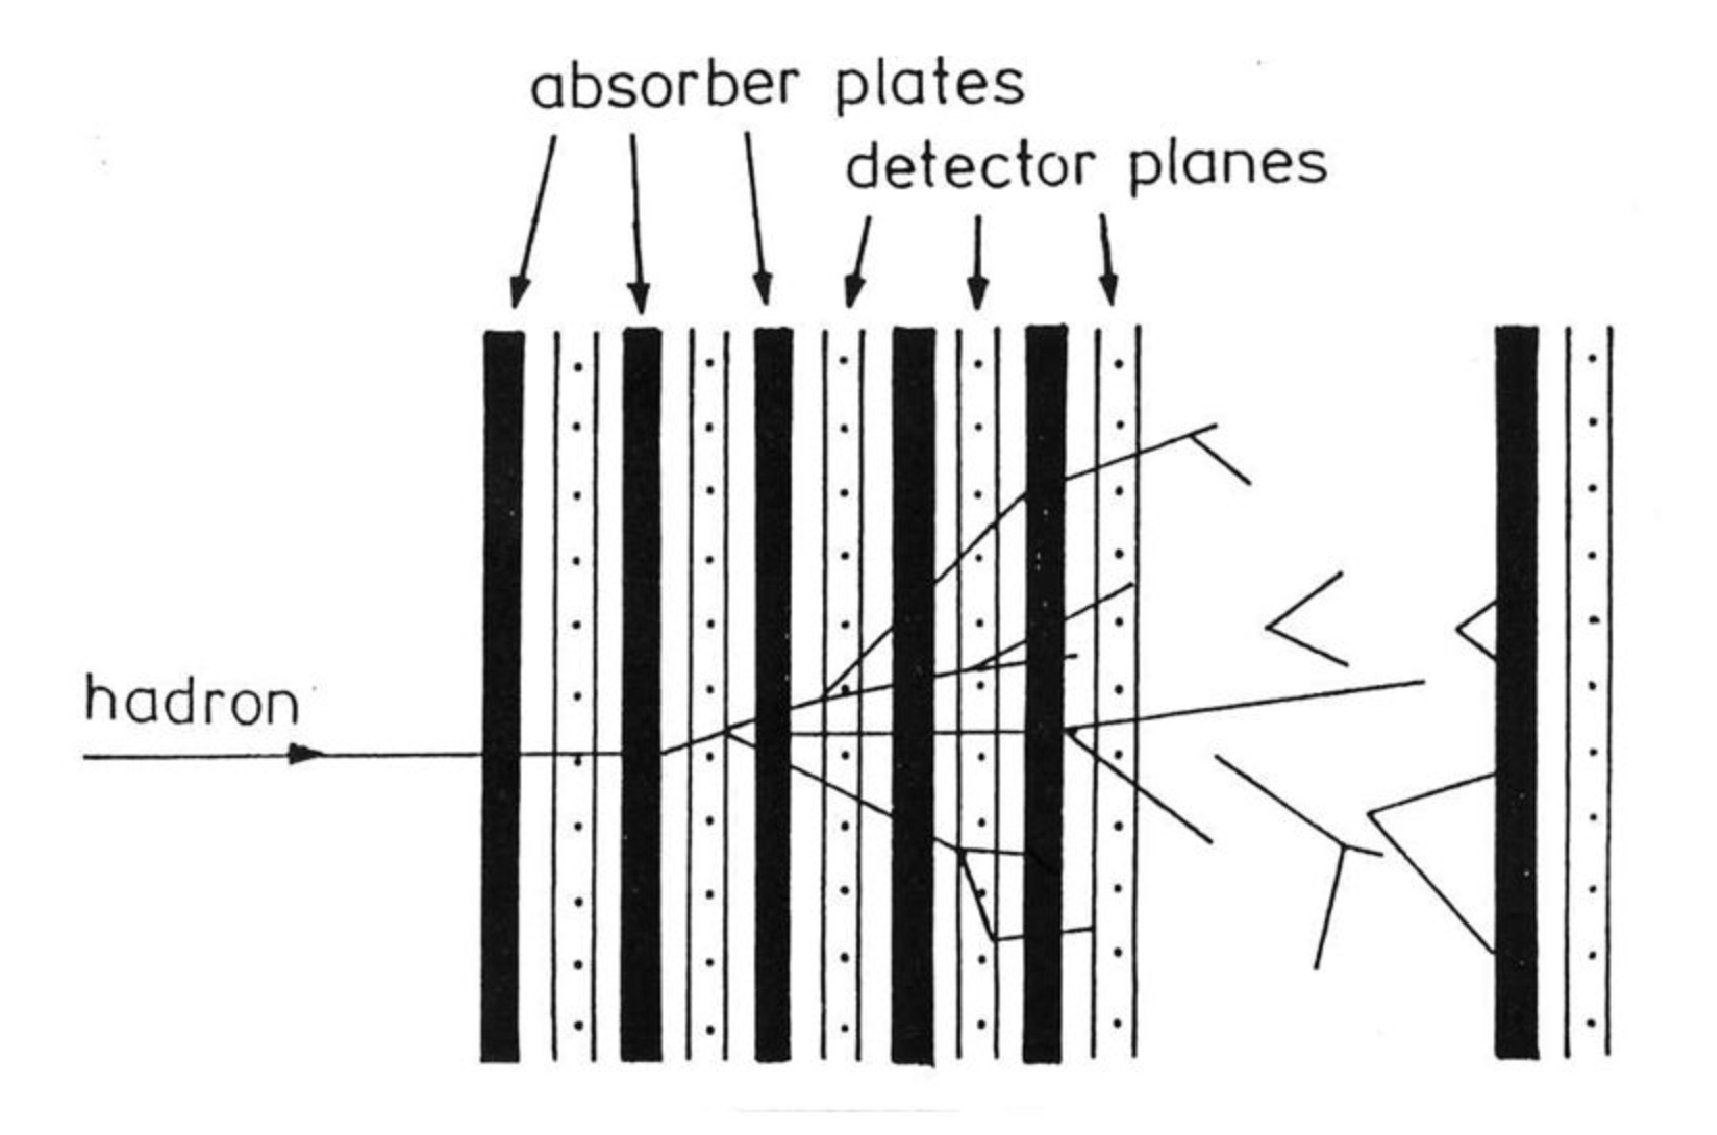
\includegraphics[width=0.5\textwidth]{Figures/sampling_calor}
	\end{enumerate}
\end{slide}

\begin{slide}[trans=Dissolve,toc=Features]{Important Parameters and Features}
    \pause
	\begin{itemize}[type=1]
		\item<2-> \myred{Linearity} of the energy measurement
		\vspace{0.3cm}
		\item <3-> \myred{Precision} of the energy measurement (resolution, $\Delta E/E$)\\\vspace{0.2cm}
		in general limited by fluctuations in the shower process\\\vspace{0.2cm}
		worse for sampling calorimeters as compared to homogeneous calorimeters
		\vspace{0.3cm}
		\item <4-> \myred{Uniformity} of the energy response to different particles (\mygreen{``e/h response''})\\\vspace{0.2cm}
		in general: response of calorimeters is different to electromagnetically interacting particles (e, $\gamma$) and hadrons (h)
		\vspace{0.3cm}
		\item <5->\myred{Good energy resolution} at high energy: the relative energy resolution decreases as 1/$\sqrt{E}$ (as opposed to momentum tracking - increases linearly)
		\vspace{0.3cm}
		\item <6->\myred{Hermeticity}: calorimeters can be built nearly as 4$\pi$-detectors (important for missing energy)
		\vspace{0.3cm}
		\item <7->\myred{Trigger/timing capabilities}: ATLAS and CMS fast (Level-1) trigger signals from calorimeters and fast muon trigger stations
	\end{itemize}
\end{slide}

\section{Electromagnetic Calorimeters}
\begin{wideslide}[trans=Fly,toc=]{Electromagnetic Calorimeters}
	\twocolumn[lcolwidth=0.75\linewidth,rcolwidth=0.25\linewidth]
	{At high $E$ bremsstrahlung and pair production dominate}
	{\includegraphics[width=\linewidth]{Figures/em_calorimeter}}
	All electromagnetic processes:
	\begin{itemize}
		\twocolumn[lcolwidth=0.35\linewidth,rcolwidth=0.35\linewidth]
		{
			\item<1-> ionisation-excitation
			\item<1-> bremsstrahlung
			\item<1-> Cherenkov
		}
		{
			\item<1-> photo-effect
			\item<1-> Compton
			\item<1-> Pair production
		}
	\end{itemize}
	\begin{itemize}
		\item<2-> Particle showers created by electrons/positrons or photons are called electro- magnetic showers (only electromagnetic interaction involved)
		\item<3-> Basic processes for particle creation: bremsstrahlung and pair creation
		\item<4-> Characteristic interaction length: radiation length $X_0$
		\item<5-> Number of particles in the shower increases, until the critical energy $E_c$ is reached; For $E < E_c$ the energy loss due to ionization and excitation dominates \ra
		the number of particles decreases, due to stopping in material
	\end{itemize}
\end{wideslide}

\begin{slide}[trans=Fly,toc=]{Electromagnetic Processes}
	\begin{figure}
		\includegraphics[width=\linewidth]{Figures/reminder_1}
	\end{figure}
\end{slide}

\begin{slide}[trans=Fly,toc=]{Electromagnetic Processes}
	\begin{figure}
	\includegraphics[width=\linewidth]{Figures/reminder_2}
\end{figure}	
\end{slide}

\begin{slide}[trans=Fly,toc=Longitudinal shower shape]{Electromagnetic Shower - Longitudinal development}
	The longitudinal shower formation is usually calculated with detailed Monte Carlo simulation, taking into account the proper interaction processes and their energy dependence;\\
	\vspace{0.4cm}
	A simple model, to illustrate the relations given below:
	\twocolumn[lcolwidth=0.55\linewidth,rcolwidth=0.45\linewidth]
	{\begin{itemize}
		\item The longitudinal energy deposition can be well described by the relation
		\begin{equation}
			\frac{dE}{dt}=E_0t^\alpha\mbox{e}^{-\beta t}
		\end{equation}
		\begin{itemize}
			\item $t$: shower depth in units of $X_0$
			\item $\alpha$, $\beta$ free parameters
			\item $t^\alpha$: at small depth number of secondaries increases
			\item $\mbox{e}^{-\beta t}$ at large depth absorption dominate
		\end{itemize}
		\item For example: E=2 GeV/c$^2$ \ra $\alpha\sim2$, $\beta\sim0.5$, $t_{max}=\alpha/\beta$
	\end{itemize}
	}
	{
		\includegraphics[width=\linewidth]{Figures/longi_shower}
	}
\end{slide}

\begin{slide}[trans=Fly,toc=]{Electromagnetic Shower - Longitudinal development}
	A more precise formulation:
	\begin{equation}
		\frac{dE}{dt}=E_0\cdot\beta\cdot\frac{(\beta t)^{\alpha-1}\mbox{e}^{-\beta t}}{\Gamma(\alpha)}
	\end{equation}
	\begin{itemize}
		\item As before for small $t$ (beginning of the shower): the particle multiplicity and thereby the deposited energy grows
		\item At the end of the shower, the number of particles and thereby the energy deposition decreases since absorptive processes (Compton and photo effect for photons, stopping of electrons by $dE/dx$ due to ionization) dominate
		\item The shower maximum is found to grow logarithmically with the energy $E_0$ of the incident particle
		\twocolumn[lcolwidth=0.5\linewidth,rcolwidth=0.5\linewidth]
		{\begin{equation*}
			t_{max}=\frac{\alpha-1}{\beta}=\ln\left(\frac{E_0}{E_c}\right)+C_{e\gamma}
		\end{equation*}
		}
		{
			\begin{eqnarray*}
				C_{e\gamma} & = & +0.5\mbox{ $\gamma$-induced showers}\\
				C_{e\gamma} & = & -0.5\mbox{ e$^\pm$-induced showers}
			\end{eqnarray*}
		}
		\myred{important practical implication: calorimeters grow only logarithmically with the energy of the particles to be absorbed}
	\end{itemize}
\end{slide}

\begin{slide}[trans=Fly,toc=Lateral shower profile]{Electromagnetic Shower - Lateral profile}
	The lateral shower profile is dominated by two processes:
	\begin{itemize}
		\item [-] Multiple Coulomb scattering
		\item [-] Relatively long free path length of low energy photons\\
		(It should be noted that the opening angle of the two particles for bremsstrahlung and pair production is very small at high energies ~ 1/$\gamma^2$)
	\end{itemize}
	\twocolumn[lcolwidth=0.6\linewidth,rcolwidth=0.4\linewidth]
	{
	The lateral width of the shower increases with the depth of the shower\\
	\vspace{0.2cm}
	(lower energy photons and electrons, multiple scattering effects are larger, long path length)\\
	\vspace{0.4cm}
	The lateral shower profile is characterized by the so-called Moliere radius $\rho_M$\\
	\vspace{0.4cm}
	About 95\% (90\%) of the shower energy are contained within a cylinder with radius $r = 2 \rho_M$ ($r = 1 \rho_M$) \ra \mygreen{well collimated!}
	}
	{
		\begin{center}
			\includegraphics[width=0.9\linewidth]{Figures/lateral_shower}
		\end{center}
			{\small Radial distr. of the energy deposited by 10 GeV e$^-$ in Cu}
	}
\end{slide}

\begin{slide}[trans=Fly,toc=]{Electromagnetic Shower - Lateral profile}
	Example: Electromagnetic showers in lead glass (OPAL detector at LEP)
	\begin{tcolorbox}
		\begin{itemize}
			\item $X0 \approx 2$ cm, EC = 11.8 MeV, $\rho_M = 1.8 X_0 \approx 3.6$ cm
			\item For $E_0 = 100$ GeV one obtains:
			\item $t_{max} \approx 13$
			\item Longitudinal containment: $t_{95\%} \approx 23 = 46$ cm
			\item Lateral containment: $R_{95\%} = 2 \rho_M = 7.2$ cm
		\end{itemize}
	\end{tcolorbox}

The compact electromagnetic showers explain the dimensions (thickness and lateral granularity) of the electromagnetic calorimeters\\
\vspace{0.5cm} \ra perfect e/$\gamma$ ID criteria: compact collimated showers
\begin{itemize}
	\item [-] small lateral shower radii
	\item [-] very small leakage into the hadronic compartment of the calorimeter
\end{itemize}
\end{slide}

\section{Hadronic Calorimeters}
\begin{slide}[trans=Fly]{Hadronic Calorimeters}
	\twocolumn[lcolwidth=0.55\linewidth,rcolwidth=0.45\linewidth]
	{
		\begin{itemize}
			\item Hadrons initiate their energy showers by inelastic hadronic interactions; (strong interaction, showers are called hadronic showers)
			\item Hadronic showers are much more complex then electromagnetic showers
			\item Several secondary particles, meson production, multiplicity increases with energy $\sim \ln(E)$\\
			The secondary hadrons undergo further inelastic collisions until their energy falls below the pion production threshold
		\end{itemize}
	}
	{
		\includegraphics[width=\textwidth]{Figures/hadr_calorimeter}
	}
	$\pi^0$ components, $\pi_0 \rightarrow \gamma\gamma$, electromagnetic sub-showers;\\
	The fraction of the electromagnetic component grows with energy,\\
	$f_{em} = 0.1 \ln E$ ($E$ in GeV, in the range 10 GeV $< E <$ 100 GeV)\\
	\vspace{0.3cm}
	Also: \myred{excited nuclei} and \mygreen{decays of particles} give rise to \myred{missing energy}
\end{slide}

\begin{slide}[trans=Fly,toc=]{Missing Energy}
\begin{itemize}
	\item During the hadronic interactions atomic nuclei are broken up or remain in exited states\\
	The corresponding energy (excitation energy, binding energy) comes from the original particle energy
	\ra no or only partial contribution to the visible energy\\	
	{\small(de-excitation has time constant, might be larger than electronic signal shaping time)}
	\item Important neutron component:\\
	The interaction of neutrons depends strongly on their energy\\
	Extreme cases:
	\begin{itemize}
		\item Nuclear reaction, e.g. nuclear fission \ra energy recovered
		\item Escaping the calorimeter (undergo only elastic scattering, without inelastic interaction)
	\end{itemize}
	\item Decays of particles (as described above, e.g. $\pi\rightarrow\mu\nu_\mu$) \ra escaping particles \ra \myred{missing energy}
\end{itemize}
\begin{tcolorbox}
	{\small These energy loss processes have important consequences:
	In general, the response of the calorimeter to electrons/photons and hadrons
	is different ! The signal for hadrons is non-linear and smaller than the e/$\gamma$ signal for the same particle energy}
\end{tcolorbox}
\end{slide}

\end{document}